\documentclass{standalone}
\usepackage{tikz}
\usetikzlibrary{positioning, arrows.meta}

% Define styles
\tikzstyle{io} = [rectangle, draw, minimum width=3.5cm, minimum height=1cm, fill=gray!20, font=\small]
\tikzstyle{block} = [rectangle, draw, minimum width=3cm, minimum height=1.4cm, fill=blue!10, font=\small]
\tikzstyle{bottleneck} = [rectangle, draw, minimum width=3cm, minimum height=1.4cm, fill=purple!15, font=\small]
\tikzstyle{arrow} = [thick, ->, >=stealth]
\tikzstyle{skip} = [thick, dotted, ->, >=stealth, gray]
\tikzstyle{textlabel} = [font=\small]

\begin{document}
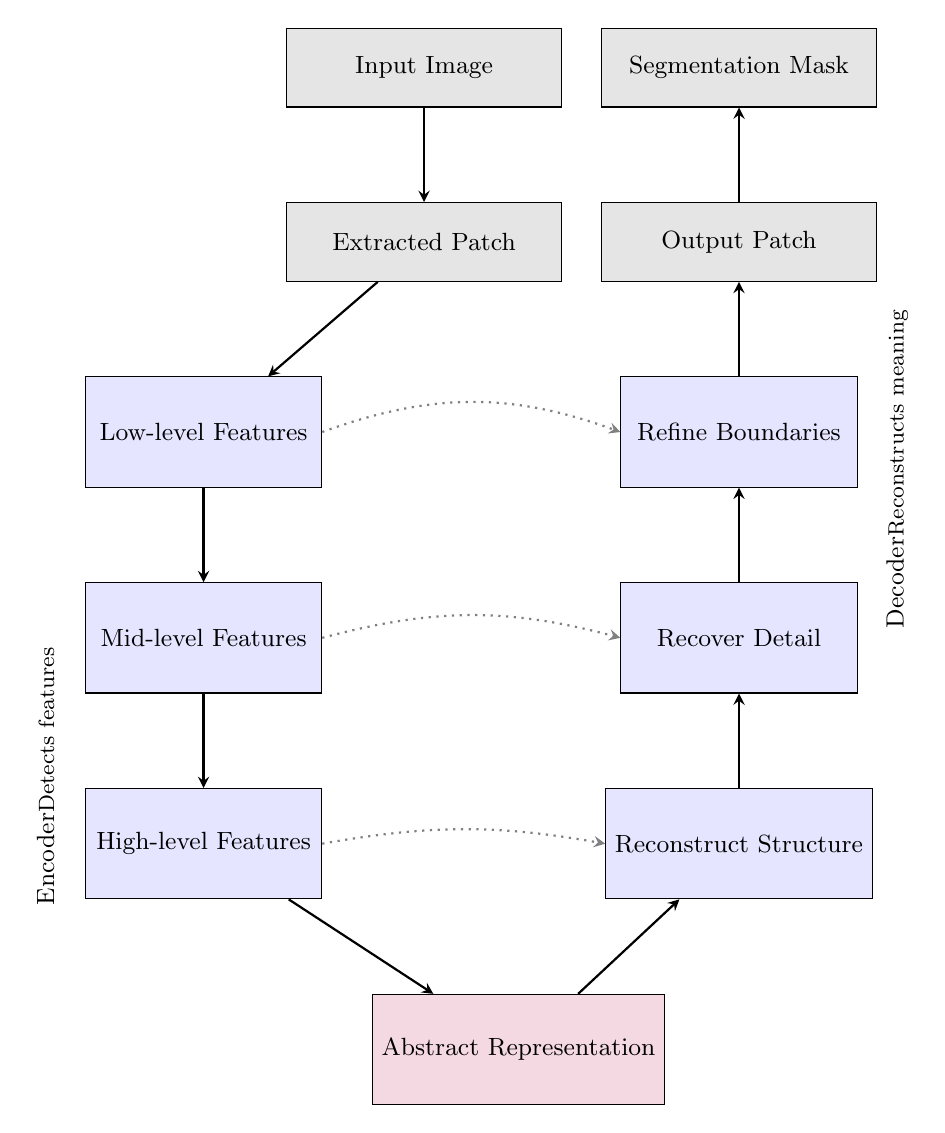
\begin{tikzpicture}[node distance=1.2cm and 2cm]

  % Input stack
  \node (input_img) [io] {Input Image};
  \node (input_patch) [io, below=of input_img] {Extracted Patch};

  % Encoder path (vertical stack)
  \node (enc1) [block, below=of input_patch, xshift=-2.8cm] {Low-level Features};
  \node (enc2) [block, below=of enc1] {Mid-level Features};
  \node (enc3) [block, below=of enc2] {High-level Features};

  % Bottleneck
  \node (bottleneck) [bottleneck, below=of enc3, xshift=4cm] {Abstract Representation};

  % Decoder path (mirrored vertical stack)
  \node (dec3) [block, above=of bottleneck, xshift=2.8cm] {Reconstruct Structure};
  \node (dec2) [block, above=of dec3] {Recover Detail};
  \node (dec1) [block, above=of dec2] {Refine Boundaries};

  % Output stack
  \node (output_patch) [io, above=of dec1] {Output Patch};
  \node (output_img) [io, above=of output_patch] {Segmentation Mask};

  % Arrows (main flow)
  \draw[arrow] (input_img) -- (input_patch);
  \draw[arrow] (input_patch) -- (enc1);
  \draw[arrow] (enc1) -- (enc2);
  \draw[arrow] (enc2) -- (enc3);
  \draw[arrow] (enc3) -- (bottleneck);
  \draw[arrow] (bottleneck) -- (dec3);
  \draw[arrow] (dec3) -- (dec2);
  \draw[arrow] (dec2) -- (dec1);
  \draw[arrow] (dec1) -- (output_patch);
  \draw[arrow] (output_patch) -- (output_img);

  % Skip connections (dotted)
  \draw[skip] (enc1.east) to[bend left=20] (dec1.west);
  \draw[skip] (enc2.east) to[bend left=15] (dec2.west);
  \draw[skip] (enc3.east) to[bend left=10] (dec3.west);

  % Side labels
  \node[textlabel, rotate=90, left=0.5cm of enc2] {Encoder\\\footnotesize Detects features};
  \node[textlabel, rotate=90, right=0.5cm of dec2] {Decoder\\\footnotesize Reconstructs meaning};

\end{tikzpicture}
\end{document}
